% Vorgaben Assignment aus Studienheft SQL03
% Formatvorgaben fuer den Text
% Umfang: 8 - 10 Seiten (inkl. Abbildungen und Tabellen, aber ohne Deckblatt, % Gliederung und Literaturverzeichnis, Eidesstattliche Erklaerung)
% Zeilenabstand: 1,5
% Schriftart: frei
% Schriftgrad: 12 pt
% Variablen, physikalische Groessen und Funktionszeichen werden kursiv gedruckt.
% Korrekturrand: links: 4,5 cm, rechts 2,0 cm, oben und unten jeweils 3,0 cm
% Deckblatt: (Adresse, AKAD-E-Mail-Adresse, Immatrikulationsnummer, Modul-
% bezeichnung, Thema, Datum, Felder fÃŒr Korrektor)
% Gliederung (1 Seite)
% Literaturverzeichnis (3 - 5 Literaturquellen  z. B. Lehrbuecher, aktuelle Fachartikel recherchieren)
% Eidesstattliche Erklaerung (unterschrieben und fest eingebunden)
% Bearbeitungsdauer: 2 Monate


\documentclass[a4paper,12pt]{article}
\usepackage{german}
\usepackage[nottoc]{tocbibind} % Anzeigen des Literaturverzeichnisses im TOC
\usepackage{epsfig}
\usepackage{times}
\usepackage{supertabular}
\usepackage{wrapfig}
\usepackage{multirow}
\usepackage[onehalfspacing]{setspace}
\usepackage{listings}
\usepackage{mathptmx}
\usepackage{geometry}
\usepackage{helvet}
\usepackage{courier}
\usepackage{setspace}
\usepackage{textcomp}
\usepackage[T1]{fontenc}
\usepackage[utf8]{inputenc}
\usepackage{fancyhdr}
\usepackage{float} % Notwendig fuer figure[h]

\renewcommand{\familydefault}{\rmdefault}

\makeatother

\geometry{a4paper, left=45mm, right=20mm, top=30mm, bottom=30mm}

\begin{document}

\begin{center}

\vspace{9cm}

\Huge{Überschrift}
\vspace{1cm}
\onehalfspacing

\Large{Assignment im Modul ABC01 - \\ Vorlage \LaTeX{}}

\vspace{1cm}
\Large{Betreuer: Prof. Dr. med. Wurst \\}
\normalsize
\vspace{2cm}

Max Mustermann\\Musterstr. 1a\\12345 Musterhausen
\\
\vspace{2cm}

14. Oktober 2012

Immatrikulationsnummer: 123456

max.mustermann@akad.de
\vspace{3cm}


\includegraphics[scale=0.2]{akad_logo.png}

\end{center}

\clearpage

\normalsize

\begin{spacing}{1.0} % Verzeichnisse werden mit einzeiligem Abstand gesetzt
\tableofcontents % Inhaltsverzeichnis
\listoffigures % Abbildungsverzeichnis
\listoftables % Tabellenverzeichnis
\end{spacing} 

\clearpage


\pagestyle{fancy}
\fancyhead{}
\fancyhead[LO,RE]{\textsc{Überschrift überall}}
\fancyhead[RO,LE]{\thepage}
\fancyfoot[CO,CE]{}

\nocite{*} 

\setcounter{page}{1}


\section{Einf"uhrung}
\subsection{Aufgabenstellung}

Lorem ipsum dolor sit amet, consetetur sadipscing elitr, sed diam nonumy eirmod tempor invidunt ut labore et dolore magna aliquyam erat, sed diam voluptua. At vero eos et accusam et justo duo dolores et ea rebum. Stet clita kasd gubergren, no sea takimata sanctus est Lorem ipsum dolor sit amet. Lorem ipsum dolor sit amet, consetetur sadipscing elitr, sed diam nonumy eirmod tempor invidunt ut labore et dolore magna aliquyam erat, sed diam voluptua. At vero eos et accusam et justo duo dolores et ea rebum. Stet clita kasd gubergren, no sea takimata sanctus est Lorem ipsum dolor sit amet.

\subsection{Ziel der Arbeit}

Lorem ipsum dolor sit amet, consetetur sadipscing elitr, sed diam nonumy eirmod tempor invidunt ut labore et dolore magna aliquyam erat, sed diam voluptua. At vero eos et accusam et justo duo dolores et ea rebum. Stet clita kasd gubergren, no sea takimata sanctus est Lorem ipsum dolor sit amet. Lorem ipsum dolor sit amet, consetetur sadipscing elitr, sed diam nonumy eirmod tempor invidunt ut labore et dolore magna aliquyam erat, sed diam voluptua. At vero eos et accusam et justo duo dolores et ea rebum. Stet clita kasd gubergren, no sea takimata sanctus est Lorem ipsum dolor sit amet.

\subsection{Aufbau}

Lorem ipsum dolor sit amet, consetetur sadipscing elitr, sed diam nonumy eirmod tempor invidunt ut labore et dolore magna aliquyam erat, sed diam voluptua. At vero eos et accusam et justo duo dolores et ea rebum. Stet clita kasd gubergren, no sea takimata sanctus est Lorem ipsum dolor sit amet. Lorem ipsum dolor sit amet, consetetur sadipscing elitr, sed diam nonumy eirmod tempor invidunt ut labore et dolore magna aliquyam erat, sed diam voluptua. At vero eos et accusam et justo duo dolores et ea rebum. Stet clita kasd gubergren, no sea takimata sanctus est Lorem ipsum dolor sit amet.

\section{Grundlagen}
\subsection{Text}

Text 

%\noindent Keine Eintrückung 

\textbf{Fett}

\textit{Kursiv}

\underline{Unterstrichen}

\subsubsection{Fußnote}

Text mit Fußnote \footnote{Die Fußnote zum Text} 


\subsubsection{Tabelle}

\begin{center}
\tablehead{ \textbf{Head1} & \textbf{Head2} & \textbf{Head3}
\\ }
\bottomcaption{\small{Beschreibung. Quelle: Internet}}
\begin{supertabular}{c|c|c}
\hline
1 & 2 & 3 \\
1 & 2 & 3 \\
1 & 2 & 3 \\
1 & 2 & 3 \\
1 & 2 & 3 \\
1 & 2 & 3 \\
1 & 2 & 3 \\
1 & 2 & 3 \\
\end{supertabular}
\end{center}

\subsection{Zitate}

Dies ist ein ganz kurzer Beispieltext \cite{Baeumle-Courth2004}. Und noch ein weites Zitat \cite{Torvalds2001}
\\
http://www.literatur-generator.de/

\subsubsection{Aufzählung}

\begin{itemize}
\item\textit{Punkt 1:} Text
\item Punkt 2: Text
\item Punkt 3: \\ Text
\end{itemize}

\subsubsection{Bilder}

\begin{figure}[H]
\begin{center}
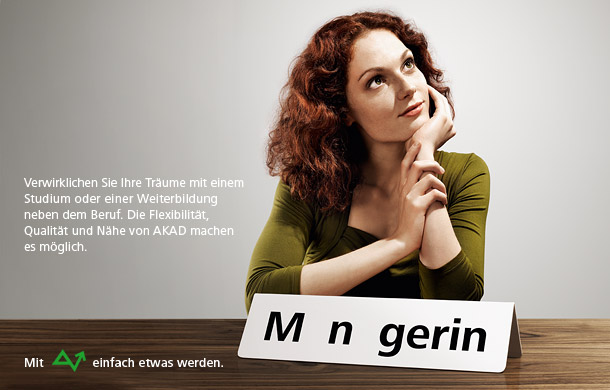
\includegraphics[scale=0.5]{akad_bild1.jpg}
\caption{Akad}
\end{center}
\end{figure}

\section{Hauptteil}

\section{Zusammenfassung}

Lorem ipsum dolor sit amet, consetetur sadipscing elitr, sed diam nonumy eirmod tempor invidunt ut labore et dolore magna aliquyam erat, sed diam voluptua. At vero eos et accusam et justo duo dolores et ea rebum. Stet clita kasd gubergren, no sea takimata sanctus est Lorem ipsum dolor sit amet. Lorem ipsum dolor sit amet, consetetur sadipscing elitr, sed diam nonumy eirmod tempor invidunt ut labore et dolore magna aliquyam erat, sed diam voluptua. At vero eos et accusam et justo duo dolores et ea rebum. Stet clita kasd gubergren, no sea takimata sanctus est Lorem ipsum dolor sit amet.


\bibliographystyle{apalike}
%\bibliographystyle{alpha}
\bibliography{literatur}


\pagestyle{empty} 

\onehalfspacing

\thispagestyle{empty}
\clearpage
\begin{center}
{\Large Eidesstattliche Erkl"arung}
\vspace*{4cm}\end{center}
\noindent
Ich versichere, dass ich das beiliegende Assignment selbstst"andig verfasst, keine anderen als die angegebenen Quellen und Hilfsmittel benutzt sowie alle w"ortlich oder sinngem"a"s "ubernommenen Stellen in der Arbeit gekennzeichnet habe. 
\vspace{3cm}

\hspace{-0.8cm}
\rule[0.5ex]{6.5cm}{1pt}
\hspace{1.3cm}
\rule[0.5ex]{6.5cm}{1pt}
(Datum, Ort)
\hspace{6.3cm}(Unterschrift)

\end{document}

